% Hlavicka pro protokoly z fyzikalniho praktika.
% Verze pro: LaTeX
% Verze hlavicky: 22. 2. 2007
% Autor: Ustav fyziky kondenzovanych latek
% Ke stazeni: www.physics.muni.cz/ufkl/Vyuka/
% Licence: volne k pouziti, nejlepe k vcasnemu odevzdani protokolu z Vaseho mereni.


\documentclass[czech,11pt,a4paper]{article}
\usepackage[T1]{fontenc}
\usepackage{graphicx}
\usepackage{mathtools}
\usepackage{amssymb}
\usepackage{amsthm}
\usepackage{thmtools}
\usepackage{xcolor}
\usepackage{nameref}
\usepackage{babel}
\usepackage{hyperref}
\usepackage{multicol}
\usepackage[export]{adjustbox}
\usepackage{subcaption}
\usepackage{caption}
\usepackage{multirow}
\usepackage{float}
\usepackage{placeins}




%%% Nemente:
\usepackage[margin=2cm]{geometry}
\newtoks\jmenopraktika \newtoks\jmeno \newtoks\datum
\newtoks\obor \newtoks\skupina \newtoks\rocnik \newtoks\semestr
\newtoks\cisloulohy \newtoks\jmenoulohy
\newtoks\tlak \newtoks\teplota \newtoks\vlhkost
%%% Nemente - konec.


%%%%%%%%%%% Doplnte pozadovane polozky:

\jmenopraktika={Fyzikální praktikum 1}  % nahradte jmenem vaseho predmetu
\jmeno={Teodor Duraković}            % nahradte jmenem mericiho
\datum={10.~března 2024}        % nahradte datem mereni ulohy
\obor={F}                     % nahradte zkratkou vami studovaneho oboru
\skupina={St 8:00}            % nahradte dobou vyuky vasi seminarni skupiny
\rocnik={I}                  % nahradte rocnikem, ve kterem studujete
\semestr={II}                 % nahradte semestrem, ve kterem studujete

\cisloulohy={10}               % nahradte cislem merene ulohy
\jmenoulohy={Tepelná vodivost pevných látek} % nahradte jmenem merene ulohy

\tlak={99 \,\rm 316}                   % nahradte tlakem pri mereni (v hPa)
\teplota={23.2}               % nahradte teplotou pri mereni (ve stupnich Celsia)
\vlhkost={42.1}               % nahradte vlhkosti vzduchu pri mereni (v %)

%%%%%%%%%%% Konec pozadovanych polozek.


%%%%%%%%%%% Uzitecne balicky:

%%%%%% Zamezeni parchantu:
\widowpenalty 10000 \clubpenalty 10000 \displaywidowpenalty 10000
%%%%%% Parametry pro moznost vsazeni vetsiho poctu obrazku na stranku
\setcounter{topnumber}{3}	  % max. pocet floatu nahore (specifikace t)
\setcounter{bottomnumber}{3}	  % max. pocet floatu dole (specifikace b)
\setcounter{totalnumber}{6}	  % max. pocet floatu na strance celkem
\renewcommand\topfraction{0.9}	  % max podil stranky pro floaty nahore
\renewcommand\bottomfraction{0.9} % max podil stranky pro floaty dole
\renewcommand\textfraction{0.1}	  % min podil stranky, ktery musi obsahovat text
\intextsep=8mm \textfloatsep=8mm  %\intextsep pro ulozeni [h] floatu a \textfloatsep pro [b] or [t]

% Tecky za cisly sekci:
\renewcommand{\thesection}{\arabic{section}.}
\renewcommand{\thesubsection}{\thesection\arabic{subsection}.}
% Jednopismenna mezera mezi cislem a nazvem kapitoly:
\makeatletter \def\@seccntformat#1{\csname the#1\endcsname\hspace{1ex}} \makeatother


%%%%%%%%%%%%%%%%%%%%%%%%%%%%%%%%%%%%%%%%%%%%%%%%%%%%%%%%%%%%%%%%%%%%%%%%%%%%%%%
%%%%%%%%%%%%%%%%%%%%%%%%%%%%%%%%%%%%%%%%%%%%%%%%%%%%%%%%%%%%%%%%%%%%%%%%%%%%%%%
% Zacatek dokumentu
%%%%%%%%%%%%%%%%%%%%%%%%%%%%%%%%%%%%%%%%%%%%%%%%%%%%%%%%%%%%%%%%%%%%%%%%%%%%%%%
%%%%%%%%%%%%%%%%%%%%%%%%%%%%%%%%%%%%%%%%%%%%%%%%%%%%%%%%%%%%%%%%%%%%%%%%%%%%%%%

\begin{document}
	
	%%%%%%%%%%%%%%%%%%%%%%%%%%%%%%%%%%%%%%%%%%%%%%%%%%%%%%%%%%%%%%%%%%%%%%%%%%%%%%%
	% Nemente:
	%%%%%%%%%%%%%%%%%%%%%%%%%%%%%%%%%%%%%%%%%%%%%%%%%%%%%%%%%%%%%%%%%%%%%%%%%%%%%%%
	\thispagestyle{empty}
	
	{
		\begin{center}
			\sf 
			{\Large Ústav fyzikální elektroniky Přírodovědecké fakulty Masarykovy univerzity} \\
			\bigskip
			{\huge \bfseries FYZIKÁLNÍ PRAKTIKUM} \\
			\bigskip
			{\Large \the\jmenopraktika}
		\end{center}
		
		\bigskip
		
		\sf
		\noindent
		\setlength{\arrayrulewidth}{1pt}
		\begin{tabular*}{\textwidth}{@{\extracolsep{\fill}} l l}
			\large {\bfseries Zpracoval:}  \the\jmeno & \large  {\bfseries Naměřeno:} \the\datum\\[2mm]
			\large  {\bfseries Obor:} \the\obor  \hspace{40mm}  {\bfseries Skupina:} \the\skupina %
			%{\bfseries Ročník:} \the\rocnik \hspace{5mm} {\bfseries Semestr:} \the\semestr  
			&\large {\bfseries Testováno:}\\
			\\
			\hline
		\end{tabular*}
	}
	
	\bigskip
	
	{
		\sf
		\noindent \begin{tabular}{p{3cm} p{0.6\textwidth}}
			\Large  Úloha č. {\bfseries \the\cisloulohy:} \par
			\smallskip
			$T=\the\teplota$~$^\circ$C \par
			$p=\the\tlak$~Pa \par
			$\varphi=\the\vlhkost$~\%
			&\Large \bfseries \the\jmenoulohy  \\[2mm]
		\end{tabular}
	}
	
	\vskip1cm
	
	%%%%%%%%%%%%%%%%%%%%%%%%%%%%%%%%%%%%%%%%%%%%%%%%%%%%%%%%%%%%%%%%%%%%%%%%%%%%%%%
	% konec Nemente.
	%%%%%%%%%%%%%%%%%%%%%%%%%%%%%%%%%%%%%%%%%%%%%%%%%%%%%%%%%%%%%%%%%%%%%%%%%%%%%%%
	
	%%%%%%%%%%%%%%%%%%%%%%%%%%%%%%%%%%%%%%%%%%%%%%%%%%%%%%%%%%%%%%%%%%%%%%%%%%%%%%%
	%%%%%%%%%%%%%%%%%%%%%%%%%%%%%%%%%%%%%%%%%%%%%%%%%%%%%%%%%%%%%%%%%%%%%%%%%%%%%%%
	% Zacatek textu vlastniho protokolu
	%%%%%%%%%%%%%%%%%%%%%%%%%%%%%%%%%%%%%%%%%%%%%%%%%%%%%%%%%%%%%%%%%%%%%%%%%%%%%%%
	%%%%%%%%%%%%%%%%%%%%%%%%%%%%%%%%%%%%%%%%%%%%%%%%%%%%%%%%%%%%%%%%%%%%%%%%%%%%%%%
	
	
	\section{Zadání}
	Změřit tepelnou vodivost sádrokartonu. Minimalizovat tepelné ztráty a realizovat způsob měření tepelného výkonu procházejícího vodičem za ustáleného stavu.
	\section{Postup, metody měření}
	Pracujeme se dvěma deskami sádrokartonu o stejných rozměrech. Teplo dodáváme soustavě topnou fólií Omega, KH-808/10. Folie je vložena \textbf{mezi} sádrokartonové desky, teplota je měřena ve čtyřech bodech:
		\begin{figure}[H]
	\begin{center}
			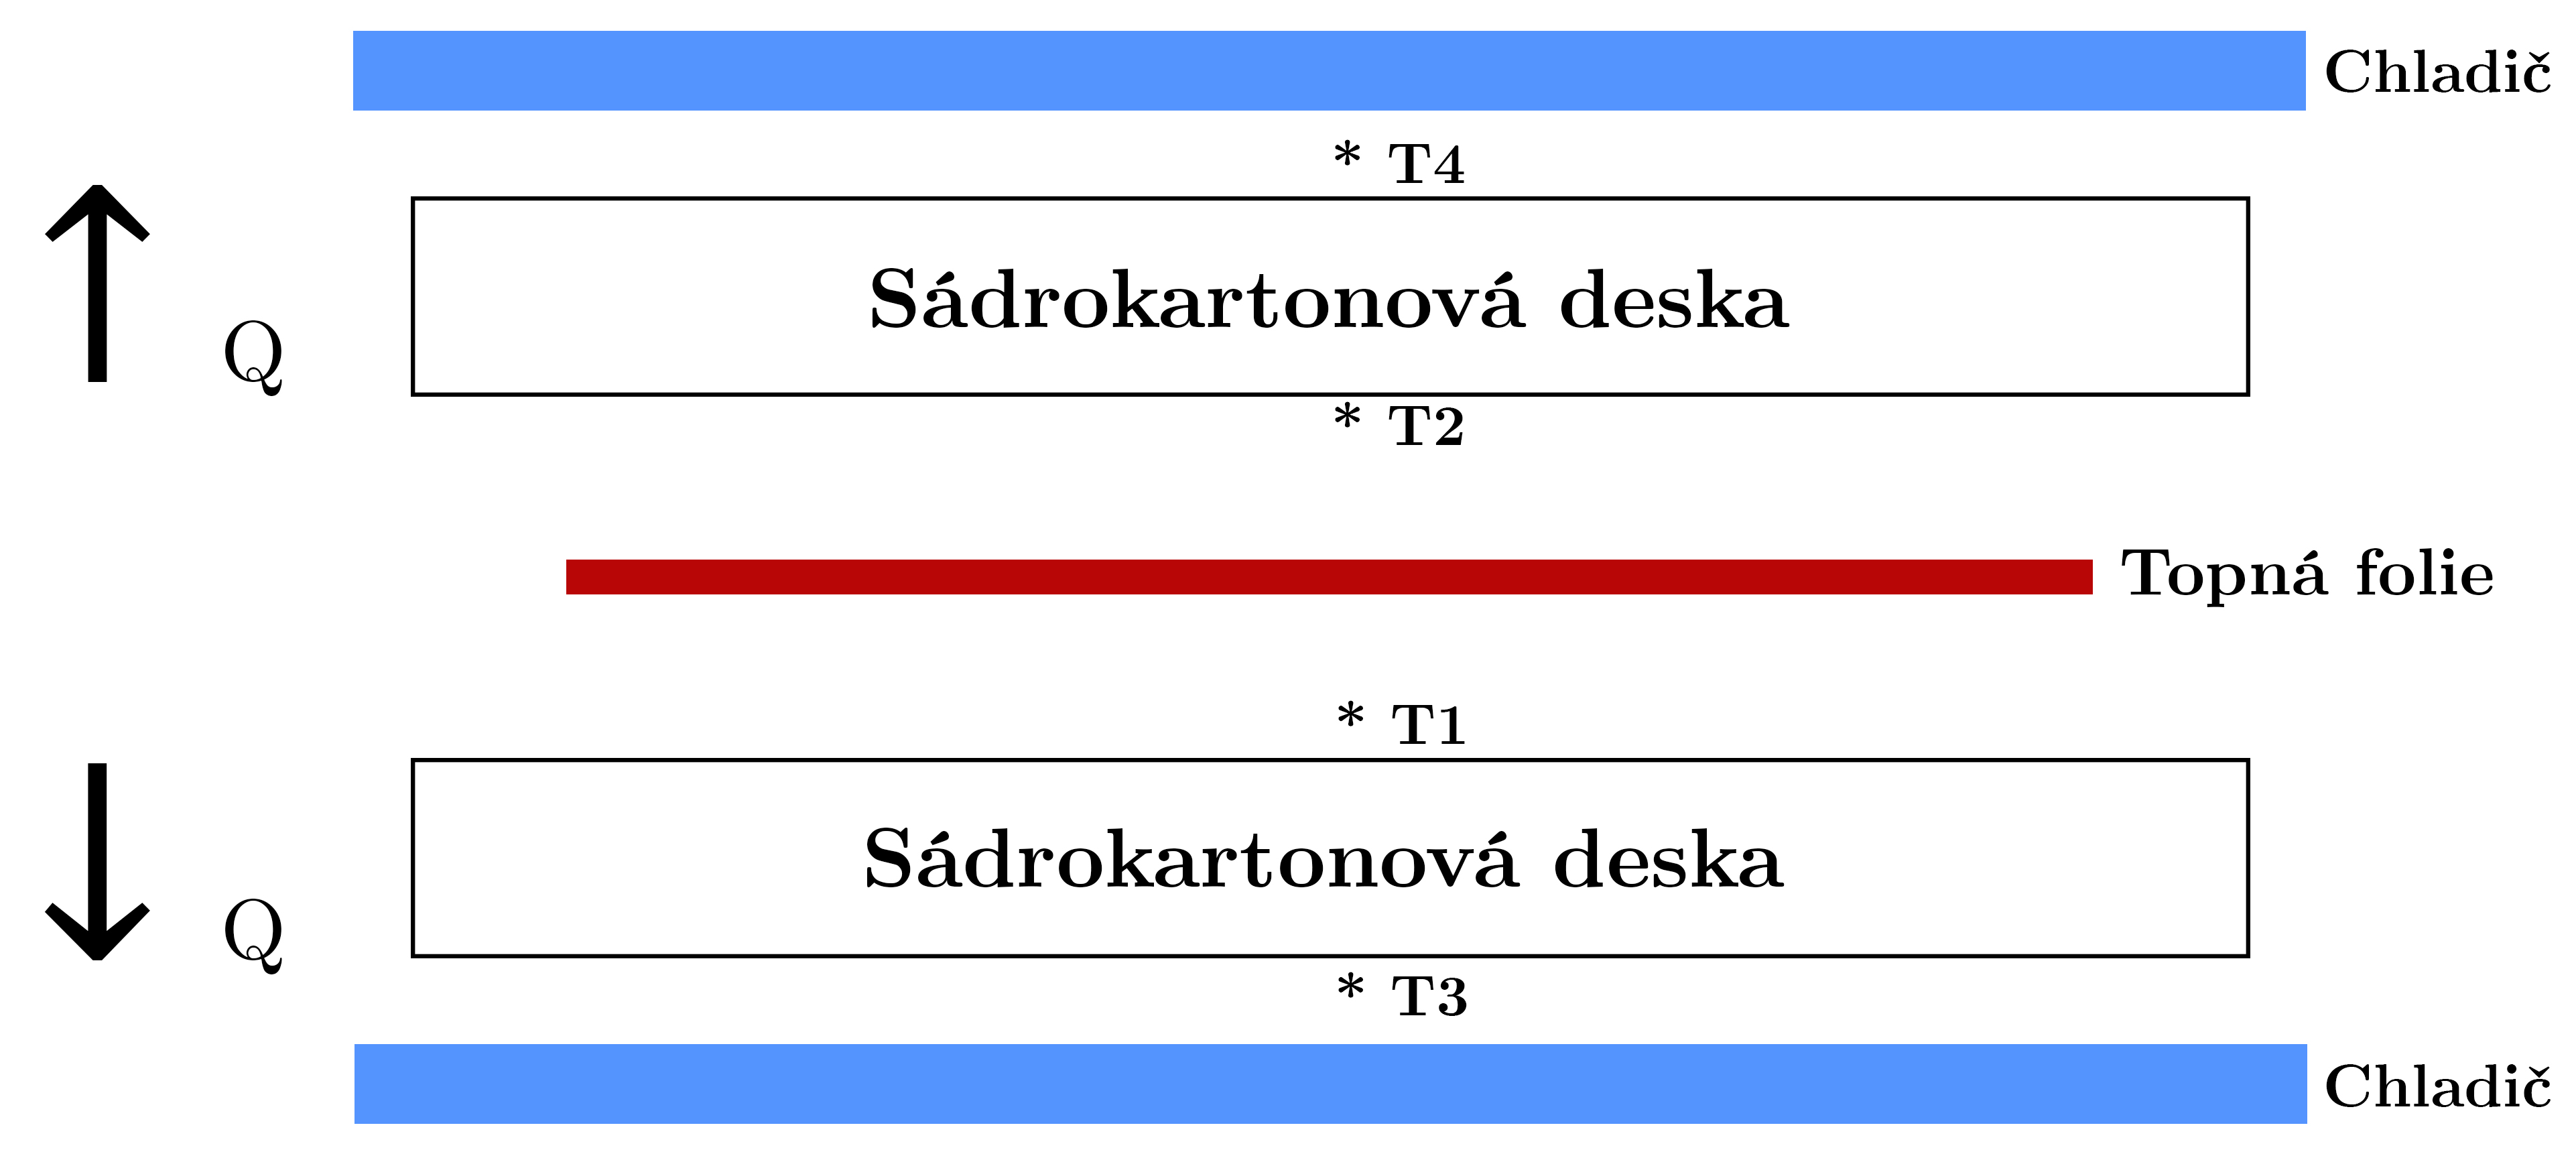
\includegraphics[width=0.7\linewidth, ]{sestava}
			\caption{Schéma realizované soustavy}
	\end{center}
	\end{figure}
\noindent Z obou stran sádrokartonové desky je vyfrézován žlábek o hloubce cca. 0.3mm vedoucí do centra desky. Do těchto žlábků jsou umístěny termočlánky typu K, kterými je teplota měřena. Při přípravě měřicí soustavy se snažíme dosáhnout co nejlepšího tepelného kontaktu mezi všemi elementy.
Topnou fólii zahříváme konstantním výkonem - měříme proud procházející folií a napětí mezi přívodními svorkami (měříme metodou A). Na čidlech $T_1, T_2$ budeme pozorovat růst teploty podléhající funkci $T_u - T_0 e^{-h \tau}$, kde $T_u$ je teplota v ustáleném stavu a $T_0$ je počáteční teplota. Ustálený stav pro nás znamená, že se folie \textbf{již dále neohřívá}, její teplota bude konstantní a tudíž pro ustálený stav můžeme říci, že veškeré přivedené teplo je odebíráno okolím, v našem případě sádrokartonovými deskami. Bude platit
\begin{gather}
	UI \tau = \lambda \frac S d(t_1 - t_2)\tau\\
	UI = \lambda \frac{S}{d} (t_1 - t_2)
\end{gather} 
kde $U,I$ jsou napětí a proud na folii, $\tau$ je čas (součin těchto členů tvoří výše zmíněné přivedené teplo), $\lambda$ je součinitel tepelné vodivosti, $S$ je obsah kolmého průřezu vodičem a $d$ je jeho délka. $t_1, t_2$ jsou teploty u ohřívače, resp. chladiče. Pro výpočet součinitele tepelné vodivosti tedy platí
\begin{equation}
	\lambda = \frac{UI}{t_1 - t_2} \frac d S
\end{equation}
Jelikož je však teplo odebíráno \textbf{dvěma deskami}, nikoliv pouze jednou, bude platit:
\begin{gather}
	Q = Q_1 + Q_2\\
	UI = \lambda \frac{S}{d} (t_1 - t_3) + \lambda  \frac{S}{d} (t_1 - t_4) = \lambda \frac{S}d \left( (t_1 - t_3) + (t_2 - t_4)\right)\\
	\lambda = \frac{UI}{(t_1 - t_3) + (t_2 - t_4)} \frac d S
\end{gather}
Pro desky sice uvažujeme stejné rozměry, očekáváme ale, že jimi odebrané teplo se \textbf{nebude} rovnat. Jeden chladič je totiž položen na umělohmotné podložce, druhý je vystaven okolí - proto očekáváme, že bude odebírat teplo okolnímu vzduchu a teplo od sádrokartonu nebude odebírat stejně efektivně jako spodní chladič.\\
Samotný experiment provedeme následovně: Zdroj nastavíme na určitý výkon a soustavu necháme přiblížit ustálenému stavu. Zapíšeme hodnoty napětí, proudu a teplot. Toto víckrát opakujeme.

\subsection{Použitá měřící technika}
	\begin{figure} [h]
		\begin{subfigure}{1\textwidth}
			\begin{center}
				
			\begin{tabular}{||l|c|c|c|c|c||}
				\hline
				& Rozsah & rozlišení & přesnost & nejistota typu B & vnitřní odpor\\
				\hline
				{Voltmetr} &$50 \,\rm V $& $1 . 10^{-3} \,\rm V$  & $\pm \, 0.02\, \%   +4$ &$\pm 0. 007\% \, + 1.3$&$10.1 \,\rm M \Omega$ \\
				\hline
				{Ampérmetr} &$4.000 \,\rm A $& $1 . 10^{-3} \,\rm A$  & $\pm \, 0.3\, \%   +3$ &$ \pm \, 0.1\, \%   +1$  &$5.3 \,\rm  \Omega$ \\
				\hline
				Teploměr (Typ K na NI9212) &cca $ 1300 \,\rm ^\circ C $& $1 . 10^{-3} \,\rm ^\circ C$ &$\pm \, 0.4 \,\rm ^\circ C$ & $\pm 0.13 \, \rm ^\circ C$& x\\ \hline
				Posuvné měřítko &x & $0.01 \,\rm mm$  & x & $0.006 \,\rm mm$ &x \\ \hline
				Mikrometr &x & $0.005 \,\rm mm$  & x & $0.003 \,\rm mm$ &x \\ \hline
				
			\end{tabular}
			\end{center}
			
			\caption*{Parametry používaných rozsahů měřících přístrojů}
		\end{subfigure}
	\end{figure}
	\newpage
	
	\section{Měření}
	\subsection{Dimenze desky}
	Pro rozměry vodičů získáváme následující údaje:
	
	\begin{center}
		\begin{tabular}{|c|c|c|c|c|}
		\hline
		&$\overline x$ [mm] & $u_a$ [mm] & $u_b$ [mm] & $u_c$ [mm] \\
		\hline
		d & 12.532 & 0.0131 & 0.003 & 0.013 \\
		\hline
		a & 201.492 & 0.113 & 0.006 & 0.113 \\
		\hline
		b & 200.136 & 0.06 & 0.006 & 0.061 \\
		\hline
	\end{tabular}
	\end{center}
	tedy:
	\begin{gather*}
		d = 12.532 \pm 0.014 \, \text{mm}, \, a = 201.49 \pm 0.12 \, \text{mm}, \, b = 200.1 \pm 0.06 \,\rm mm \\
		\nu = 9, \, p = 0.6827 
	\end{gather*}
\textit{Měřili jsme rozměry pouze jedné desky, jelikož byly obě na první i druhý pohled shledány za rozměrově téměř identické}
   \subsection{Teplota}
   Údaje o teplotě získáváme z termočlánku typu K, platí:
   \begin{gather}
   	U = \beta (T - T_{ref}) \\
   	T = \frac U \beta + T_{ref}
   \end{gather}
   kde $T_{ref}$ je referenční teplota, tj. teplota okolí, $U$ je naměřené napětí, $\beta$ Seebeckův koeficient, v případě termočlánku K platí $\beta = 42  \, \rm \mu V \cdot ^\circ C ^{-1}$  a $T$ je hledaná teplota. \\

   Získáváme:
   	
   \begin{figure}[H]
   	\begin{center}
   		
   	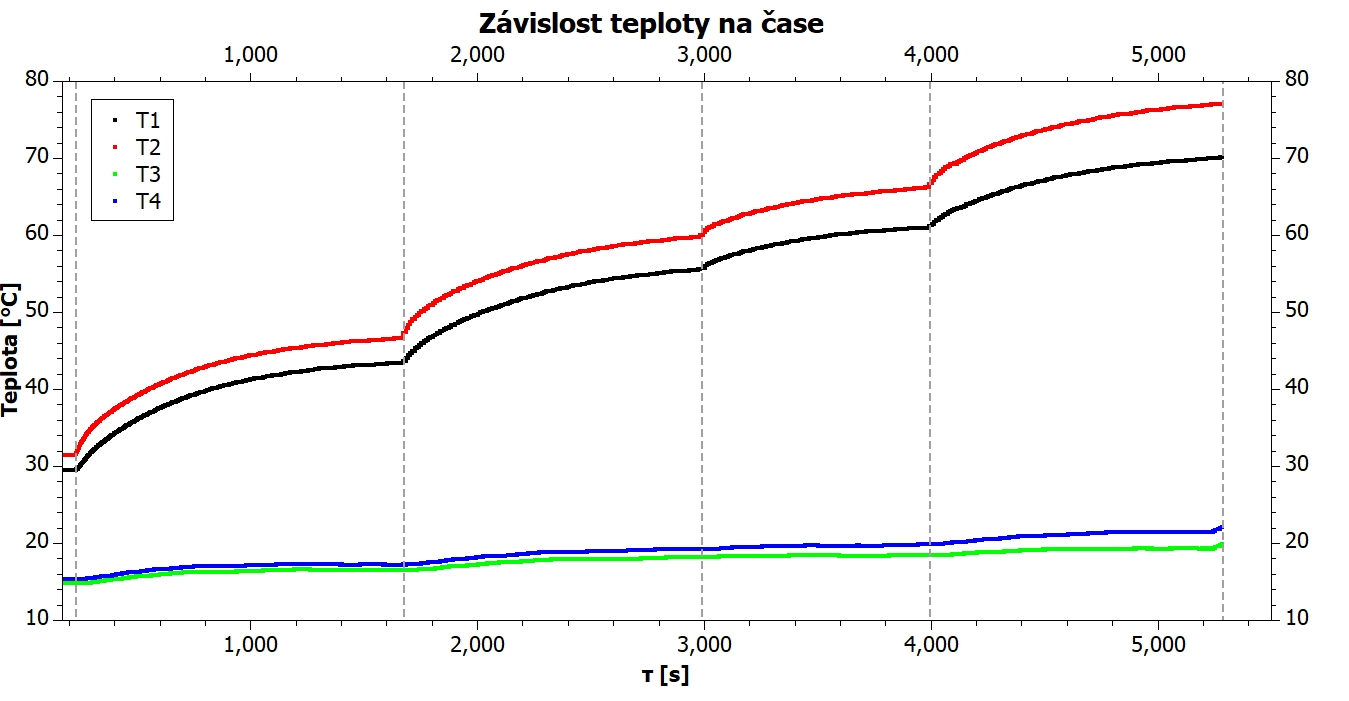
\includegraphics[width = 1\textwidth, ]{zavislost}
   	\end{center}
   \end{figure}
   
   Důležité jsou pro nás údaje v časech označených čárkovanými liniemi - \textbf{jedná se totiž o hodnoty nejbližší ústálenému stavu.} Zapisujeme tedy hodnoty pro 5 ustálených stavů.\\
   	
   \subsection{Měření proudu a napětí}
   Při dosažení ustáleného stavu je vždy odečten proud z ampérmetru a napětí z voltmetru. Jak bylo již zmíněno, hodnoty měříme při zapojení způsobem A:
   
    \begin{figure}[H]
   	\begin{center}
   		
   		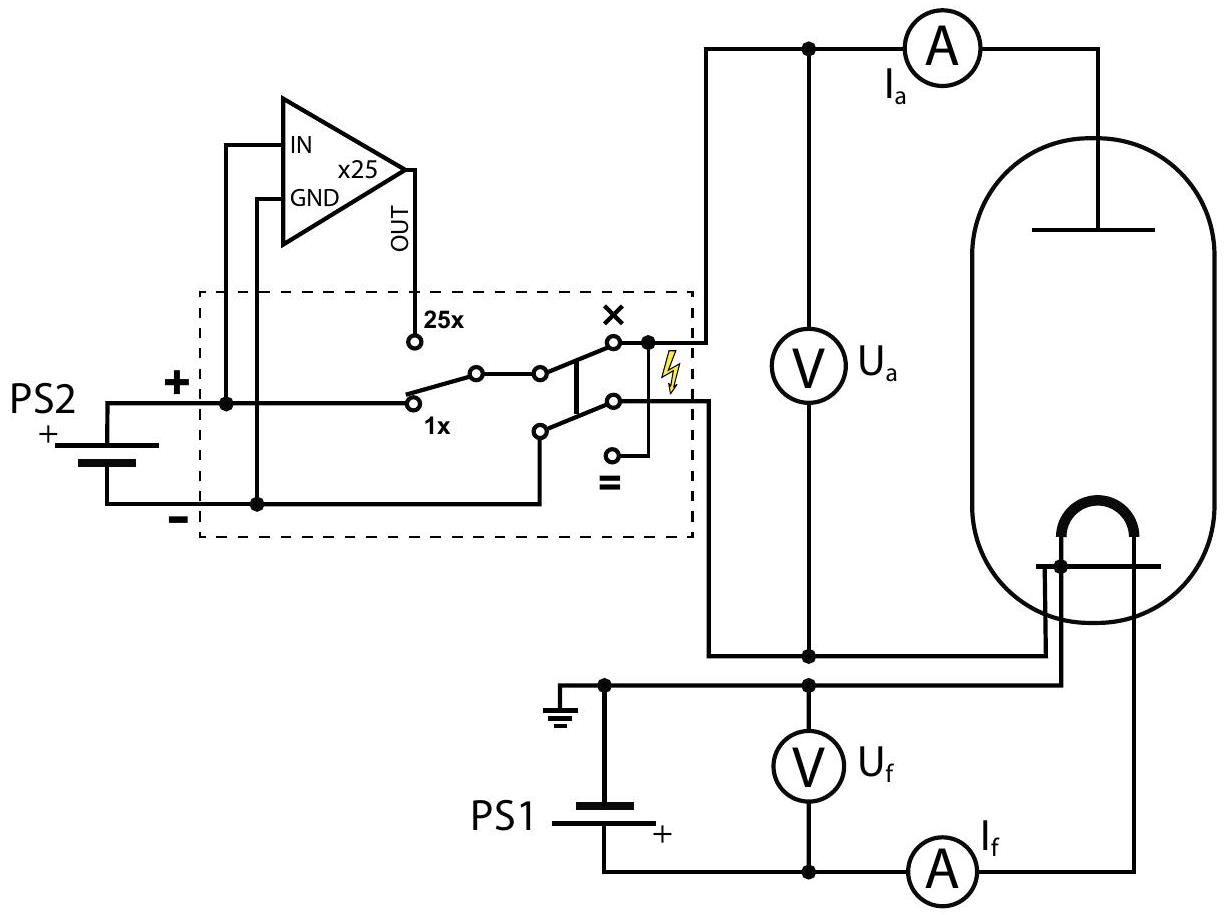
\includegraphics[width = 1\textwidth, ]{zapojeni}
   	\end{center}
   \end{figure}
   \noindent\textit{Folie je ve schématu zakreslena jako rezistor, jelikož se vlastně jedná pouze o rezistor se specifickými dimenzemi.}\\
   Při paralelním měření napětí a proudu je nutno eliminovat systematickou chybu. V našem případě je chyba přítomna při měření ampérmetru, jelikož měří proud protékající rezistorem (folií) i voltmetrem. Adjustaci provedeme aplikací formule:
   \begin{gather}
   	I_A = I + I_V\\
   	I = I_A - I_V = I_A - \frac {U_V}{R_V} 
   \end{gather}
   Pro měření v ustálených stavech získáváme:
   
  \begin{center}
  	 \begin{tabular}{|c|c|c|c|c|}
   	\hline
   	n & U [V] & I [A]& I - korekce [A]& P [W]\\
   	\hline
   	1 & $19.825 \pm 0.003$ & $ 1.021 \pm 0.002 $ & $ 1.021 \pm 0.002  $& $20.24 \pm 0.04$\\
   	\hline
   	2 & $27.148 \pm 0.003$ & $ 1.382 \pm 0.002 $  & $ 1.382 \pm 0.002 $& $37.52 \pm 0.06$\\
   	\hline
   	3 & $31.770 \pm 0.004 $& $1.617 \pm 0.003 $& $1.617 \pm 0.003 $&  $51.37 \pm 0.08$\\
   	\hline
   	4 & $33.598 \pm 0.004 $ & $1.721 \pm 0.003 $  & $1.721 \pm 0.003 $& $57.82 \pm 0.09$\\
   	\hline
   	5 & $ 36.567 \pm 0.004$ & $1.900 \pm 0.003 $ & $1.900 \pm 0.003 $ &  $ 69.47 \pm 0.11$\\
   	\hline
   \end{tabular}\\
  \end{center}
   Jelikož studujeme fyziku, místo manuálního výpočtu přístrojových nejistot jsme vynaložili ekvivalentní (ne-li větší) množství času pro výrobu skriptu, který kalkulaci výše uvedené tabulky vykonal za nás. U korigované hodnoty proudu si můžeme všimnout, že se hodnoty při použitém zaokrouhlení od původních hodnot nijak neliší. Vždy je však lepší adjustaci provést, než neprovést. \newpage
   
   \section{Výsledky}
   
   Pro 5 ustálených stavů získáváme: \\
   \begin{center}
   	\begin{tabular}{|c|c|c|c|c|c|c|}
   	\hline
   	n & P   [W]  & T1 [°C]   & T2 [°C]    & T3 [°C]   & T4 [°C]   & $\lambda \,\rm [W \, m^{-1} K^{-1}]$        \\ \hline
   	1 & 20.24 & 29.66 & 31.85 & 14.97 & 15.52 & $0.2029 \pm 0.0018$ \\ \hline
   	2 & 37.52 & 43.56 & 46.76 & 16.61 & 17.35 & $0.2069\pm 0.0011 $\\ \hline
   	3 & 51.37 & 55.70 & 59.98 & 18.31 & 19.37 & $0.2047 \pm0.0008$ \\ \hline
   	4 & 57.82 & 61.11 & 66.32 & 18.62 & 19.97 & $0.2023\pm 0.0007$ \\ \hline
   	5 & 69.48 & 70.16 & 77.14 & 19.96 & 22.16 & $0.2053 \pm 0.0007$ \\ \hline
   \end{tabular}
   \end{center}
   \begin{equation}
   	\overline{\lambda} = 0.2044 \pm 0.0005 \,\rm W \, m^{-1} K^{-1}
   \end{equation}
   
	
	\section{Závěr}
	Pro koeficient tepelné vodivosti jsme získali hodnotu, která se blíží běžně uváděné hodnotě \\
	${\lambda} = 0.22 \,\rm W \, m^{-1} K^{-1}$. Zároveň se nám nepodařilo nalézt přímý zdroj této chyby (pokud by byla způsobena tepelnými ztrátami, koeficient by byl větší, nikoliv menší). \textit{Úprava po konsultaci: za možný zdroj odchylky měřené hodnoty od hodnoty nalezené on-line byla po diskusi označena skutečnost, že samotný materiál je vyráběn v různých provedeních s mírně odlišnými hodnotami lambda, k odchylce mohla přispět i nehomogenní povaha materiálu, kvůli které se tepelná vodivost v každém bodě plochy bude mírně lišit.}
	\section{Použitý kód}
	{\tiny \begin{verbatim}
		import numpy 
		from uncertainties import *
		R = ufloat (10.1e6, 0)
		d = ufloat (12.532e-3, 0.014e-3)
		a = ufloat(201.49e-3, 0.14e-3)
		b = ufloat (200.1e-3, 0.1e-3)
		S = a*b
		
		
		
		def calc(n, rel, dig):
		calcdone = []
		for value in n:
		calc_value = float(value) * rel + dig 
		calcdone.append(calc_value)
		return calcdone
		
		
		# Pro voltmetr:
		u = [19.825,27.148,31.770,33.598,36.567]
		UERR = (0.00007) #nejistota od vyrobce, NE V PROCENTECH, ABSOLUTNE
		UDIG = (0.0013) #cast "digits" vynasobena rozslisenim 
		
		#pro ampermetr:
		i = [1.021, 1.382,1.617,1.721,1.900]
		IERR = (0.001)
		IDIG = (0.001)
		
		
		calcdone = calc(u, UERR,UDIG)
		
		print("Nejistoty napeti:", calcdone)
		u1, u2, u3, u4, u5 = [ufloat(x, y) for x, y in zip(u, calcdone)]
		uF = [ufloat(x, y) for x, y in zip(u, calcdone)]
		print ("U1 =", u1)
		print ("U2 =", u2)
		print ("U3 =", u3)
		print ("U4 =", u4)
		print ("U5 =", u5)
		
		calcdone = calc(i, IERR , IDIG)
		
		print("Nejistoty prudu:", calcdone)
		i1, i2, i3, i4, i5 = [ufloat(x, y) for x, y in zip(i, calcdone)]
		iF = [ufloat(x, y) for x, y in zip(i, calcdone)]
		print ("i1 =", i1)
		print ("i2 =", i2)
		print ("i3 =", i3)
		print ("i4 =", i4)
		print ("i5 =", i5)
		
		print("set napeti", uF)
		print("set proudu", iF)
		#ADJUSTACE AMPERMETRU:
		
		print("")
		print("\\\\\\ adjustace ampermetru\\\\\\\\")
		
		
		iCorr = []
		for u, i in zip(uF, iF):
		iCorr_value = i - u/R; 
		iCorr.append(iCorr_value)
		i1c, i2c, i3c, i4c, i5c = iCorr
		print ("i1 po korekci =", i1c)
		print ("i2 po korekci =", i2c)
		print ("i3 po korekci =", i3c)
		print ("i4 po korekci =", i4c)
		print ("i5 po korekci =", i5c)
		
		P = []
		for u, i in zip(uF, iCorr):
		P_value = u*i; 
		P.append(P_value)
		
		print (P)
		P1,P2,P3,P4,P5 = P
		print ("P1 = ", P1)
		print ("P2 = ", P2)
		print ("P3 = ", P3)
		print ("P4 = ", P4)
		print ("P5 = ", P5)
		
		
		
		T11 = ufloat (29.662,0.13)
		T12 = ufloat (31.846,0.13)
		T13 = ufloat (14.974,0.13)
		T14 = ufloat (15.523,0.13)
		
		
		#t = 1665.1
		T21 = ufloat (43.557,0.13)
		T22 = ufloat (46.763,0.13)
		T23 = ufloat (16.613,0.13)
		T24 = ufloat (17.350,0.13)
		
		
		#t3 = 2981
		T31 = ufloat (55.697,0.13)
		T32 = ufloat (59.979,0.13)
		T33 = ufloat (18.314,0.13)
		T34 = ufloat (19.372,0.13)
		
		#t = 3982
		T41 = ufloat (61.105,0.13)
		T42 = ufloat (66.317,0.13)
		T43 = ufloat (18.617,0.13)
		T44 = ufloat (19.971,0.13)
		
		#t = 5276
		T51 = ufloat (70.155,0.13)
		T52 = ufloat (77.141,0.13)
		T53 = ufloat (19.955,0.13)
		T54 = ufloat (22.156,0.13)
		
		T1 = T11, T21, T31, T41, T51
		
		T2 = T12, T22, T32, T42, T52
		
		T3 = T13, T23, T33, T43, T53
		
		T4 = T14, T24, T34, T44, T54
		lm = []
		for P, t1, t2, t3, t4 in zip(P, T1,T2,T3,T4):
		lambda_value = (P/((t1 - t3)+(t2-t4)))* d/S; 
		lm.append(lambda_value)
		
		print (lm)
		
		lm1,lm2,lm3,lm4,lm5 = lm
		print ("lambda 1 = ", lm1)
		print ("lambda 2 = ", lm2)
		print ("lambda 3 = ", lm3)
		print ("lambda 4 = ", lm4)
		print ("lambda 5 = ", lm5)
		
		print ("lambda prumer =", (lm1+lm2+lm3+lm4+lm5)/5)
	\end{verbatim}}
	% Nakonec nezapomeňte projet text programem vlna nebo vlnka, např.
	% 	vlna -m -l -n mojeuloha.tex
	% nebo zkontrolovat a opravit jednopísmenné předložky na koncích řádků ručně.
	
	
\end{document}
